% ====================================================================
% graphite_ica_ch2_v4-09.tex -- Chapter 2 v4-09 (Codex)
%   Topic: statistical thermodynamics of entropy coefficient and
%   reversible heat for graphite coin half-cell interpretation.
%   Base: v3 skeleton, expanded into distribution-explicit chapter.
%   Build: xelatex 2-pass (kotex).
% ====================================================================
\documentclass[11pt,a4paper]{article}
\usepackage[margin=22mm]{geometry}
\usepackage{kotex}
\setmonofont{D2Coding}[Scale=MatchLowercase]
\usepackage{amsmath,amssymb,mathtools,bm}
\usepackage{booktabs,longtable,array}
\usepackage{enumitem}
\usepackage{amsthm}
\usepackage{xcolor}
\usepackage{tikz}
\usetikzlibrary{arrows.meta,positioning,calc,patterns}
\usepackage{hyperref}
\usepackage{fancyhdr}
\usepackage{lastpage}
\usepackage{setspace}

\setstretch{1.12}
\setlength{\parskip}{0.45em}
\setlength{\parindent}{0pt}
\setlength{\headheight}{14pt}
\setlength{\emergencystretch}{2em}
\hypersetup{colorlinks=true, linkcolor=blue, urlcolor=blue, citecolor=blue,
  pdftitle={흑연 음극 dQ/dV -- Chapter 2 v4-09: 통계열역학 엔트로피와 가역 발열}}
\pagestyle{fancy}\fancyhf{}
\lhead{흑연 음극 $dQ/dV$ -- Ch.2 v4-09 통계열역학 엔트로피}\rhead{\thepage/\pageref{LastPage}}
\renewcommand{\headrulewidth}{0.4pt}

\newtheorem*{keybox}{핵심}
\newtheorem*{srcbox}{문헌 근거}
\newtheorem*{warnbox}{주의}
\newtheorem*{workbox}{계산 절차}

\newcommand{\dd}{\mathrm{d}}
\newcommand{\rxn}{\mathrm{rxn}}
\newcommand{\eq}{\mathrm{eq}}
\newcommand{\rev}{\mathrm{rev}}
\newcommand{\irr}{\mathrm{irr}}
\newcommand{\oc}{\mathrm{oc}}
\newcommand{\conf}{\mathrm{config}}
\newcommand{\vib}{\mathrm{vib}}
\newcommand{\el}{\mathrm{el}}
\newcommand{\eff}{\mathrm{eff}}
\newcommand{\hys}{\mathrm{hys}}
\newcommand{\Li}{\mathrm{Li}}
\newcommand{\BE}{\mathrm{BE}}
\newcommand{\FD}{\mathrm{FD}}
\newcommand{\kB}{k_\mathrm{B}}
\renewcommand{\theequation}{2.\arabic{equation}}
\renewcommand{\thesection}{2.\arabic{section}}

\title{\textbf{\LARGE Chapter 2}\\[0.35em]
\Large 흑연 음극 코인 하프셀의 엔트로피 계수와 가역 발열\\[0.2em]
\large 분배함수, 점유 분포, configurational/vibrational/electronic 엔트로피 (v4-09)}
\author{}\date{}

\begin{document}
\maketitle

\begin{abstract}
이 장은 흑연 음극 코인 하프셀의 $\partial U_\oc/\partial T$ 와 가역 발열을
``전이별 상수 몇 개''가 아니라 \emph{분포의 온도 재배열}로 해석한다. 출발점은
Chapter 1 의 logistic 전이이지만, 여기서는 그 logistic 을 단일 자리 grand-canonical
분배함수에서 다시 세운다. 이어 점유 확률 $p_0,p_1$ 로부터
$S_\conf=-R\sum p\ln p$ 를 유도하고, Bragg--Williams 상호작용 $\Omega$,
포논 Bose--Einstein 분포, 전자 Fermi--Dirac 분포를 같은 엔트로피 사슬에 놓는다.
실제 $dQ/dV$ 해석에서는 전이 겹침을 국소 peak weight 로 평균하고, 봉우리 내부
configurational 항은 logistic 폭이 이미 생성하므로 $\Delta S^0_{\rxn,j}$ 에 중복
가산하지 않는다. 범위는 단일 전극 대 Li 의 코인 하프셀 해석이며, 전셀 합성은
다루지 않는다.
\end{abstract}

\tableofcontents
\newpage

% ====================================================================
\section*{서 -- 왜 엔트로피에는 통계가 필요한가}
\addcontentsline{toc}{section}{서}
% ====================================================================
Bernardi, Pawlikowski, Newman 의 에너지 수지에서 전극의 가역 발열은
\begin{equation}
\dot Q_\rev=-I\,T\,\frac{\partial U_\oc}{\partial T}
=-\frac{I\,T}{F}\,\Delta S(x)
\label{eq:qrev_intro}
\end{equation}
로 쓴다 \cite{bernardi1985,newman}. 이 식은 익숙하지만, $\Delta S(x)$ 가 어디서
오는지 보이지 않으면 단지 경험 곡선으로 남는다. 엔트로피는 상태 하나의 이름이
아니라 \emph{가능한 미시상태들이 어떤 확률로 점유되는가}의 함수다. 따라서
흑연 staging 전위의 온도 기울기를 이해하려면 Li 자리 점유, 격자 진동, 전자
점유라는 세 분포를 먼저 세워야 한다.

Chapter 1 은 흑연 $dQ/dV$ 의 forward 모델을 전이별 logistic 종으로 표현했다. 이 장은
그 결과를 재유도하지 않고, 그 logistic 이 열역학적으로 어떤 분포인지 해석한다.
핵심 사슬은 다음이다.
\begin{equation}
\boxed{\;
Z \longrightarrow p(n) \longrightarrow \langle n\rangle=\xi_\eq
\longrightarrow S=-R\sum_i p_i\ln p_i
\longrightarrow \frac{\partial U_\oc}{\partial T}
\longrightarrow \dot Q_\rev
\;}
\label{eq:spine}
\end{equation}
즉 가역열은 ``숨은 열원''이 아니라, 전류가 한 SOC(state of charge)에서 다음 SOC 로
이동시키는 Li(+전자) 분포가 온도에 따라 다시 조직되는 열이다.

\begin{warnbox}
본 장의 전위는 흑연 전극 대 Li/Li$^+$ 기준의 코인 하프셀 평형 전위 $U_\oc$ 이다.
양극-음극 전압 차를 합성하는 전셀 식은 이 장의 범위 밖이다. LCO 는 electronic
entropy 항을 설명하는 \emph{단일 전극 하프셀 사례}로만 언급한다.
\end{warnbox}

% ====================================================================
\section{단일 자리 분배함수에서 Chapter 1 logistic 까지}
\label{sec:partition}
% ====================================================================
\subsection{Grand-canonical 두 상태 자리}
흑연의 한 삽입 자리를 가장 작게 보면 비어 있는 상태 $n=0$ 과 Li 가 점유한 상태
$n=1$ 두 상태다. 점유 상태의 자리 에너지를 $\varepsilon_0$, Li 전기화학 퍼텐셜을
$\mu$ 라 하면, 한 자리의 grand-canonical 분배함수는
\begin{equation}
Z_1=\sum_{n=0}^{1}\exp[-\beta n(\varepsilon_0-\mu)]
=1+\exp[-\beta(\varepsilon_0-\mu)],
\qquad \beta=\frac{1}{\kB T}.
\label{eq:z1}
\end{equation}
따라서 두 상태 확률은
\begin{equation}
p_0=\frac{1}{Z_1},\qquad
p_1=\frac{\exp[-\beta(\varepsilon_0-\mu)]}{Z_1}.
\label{eq:p01}
\end{equation}
점유수의 평균은 $n=1$ 확률 그 자체이므로
\begin{equation}
\langle n\rangle=p_1
=\frac{1}{1+\exp[\beta(\varepsilon_0-\mu)]}.
\label{eq:fermi_form}
\end{equation}
형식은 Fermi--Dirac 분포와 같다. 여기서 Pauli 전자를 말하는 것이 아니라, 한
삽입 자리가 동시에 두 Li 를 받을 수 없다는 0/1 점유 제약이 같은 수학을 만든다.

\subsection{전극 전위로 쓰면 logistic}
Chapter 1 의 전이 $j$ 에 대해 평형 중심 전위를 $U_j(T)$, 방향 부호를 $\sigma_d$,
$w_j=RT/F$ 라 두면 같은 점유식은
\begin{equation}
\xi_{\eq,j}(V,T)
=\frac{1}{1+\exp[-\sigma_d(V-U_j(T))/w_j]}.
\label{eq:ch1_logistic}
\end{equation}
즉 Ch1 의 logistic 은 임의로 고른 curve shape 가 아니라, 식~\eqref{eq:z1}의 두
상태 점유 분포가 전극 전위 좌표로 쓰인 것이다. $w_j=RT/F$ 는 단순 smoothing
상수가 아니라 열분포 폭이다. 온도가 올라가면 확률 분포가 넓어지고, 같은 전이
중심 주변에서 $\xi$ 가 더 완만하게 변한다.

\begin{figure}[t]
\centering
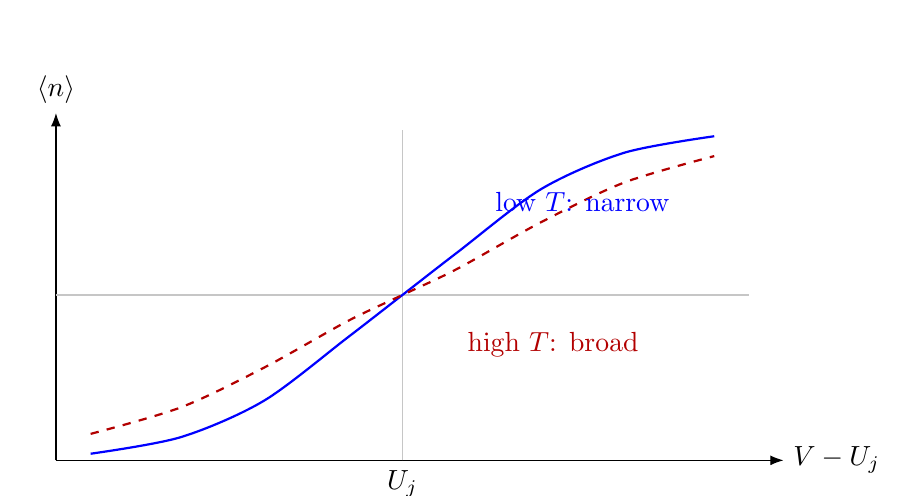
\begin{tikzpicture}[x=8.8cm,y=4.2cm,>=Latex]
  \draw[->] (0,0) -- (1.05,0) node[right] {$V-U_j$};
  \draw[->] (0,0) -- (0,1.05) node[above] {$\langle n\rangle$};
  \draw[gray!45] (0,0.5) -- (1.0,0.5);
  \draw[gray!45] (0.5,0) -- (0.5,1.0);
  \draw[thick,blue] plot[smooth] coordinates
    {(0.05,0.02) (0.18,0.07) (0.30,0.18) (0.42,0.37) (0.50,0.50)
     (0.58,0.63) (0.70,0.82) (0.82,0.93) (0.95,0.98)};
  \draw[thick,red!70!black,dashed] plot[smooth] coordinates
    {(0.05,0.08) (0.18,0.16) (0.30,0.28) (0.42,0.42) (0.50,0.50)
     (0.58,0.58) (0.70,0.72) (0.82,0.84) (0.95,0.92)};
  \node[blue,anchor=west] at (0.62,0.78) {low $T$: narrow};
  \node[red!70!black,anchor=west] at (0.58,0.35) {high $T$: broad};
  \node[below] at (0.5,0) {$U_j$};
\end{tikzpicture}
\caption{A Ch1 logistic transition is a two-state occupation distribution written in voltage coordinates.}
\label{fig:logistic}
\end{figure}

\subsection{Bragg--Williams 평균장과 상호작용}
독립 자리이면 식~\eqref{eq:fermi_form}으로 충분하지만, staging 은 인접 점유와
공공(空孔)의 상호작용을 갖는다. 평균장 자유에너지를 자리 1몰 기준으로 쓰면
\begin{equation}
g(\theta,T)=g_0(\theta,T)
 +RT\{\theta\ln\theta+(1-\theta)\ln(1-\theta)\}
 +\Omega\,\theta(1-\theta),
\label{eq:bw}
\end{equation}
여기서 $\theta$ 는 Li 점유율, $\Omega$ 는 정규용액 상호작용 parameter 다
\cite{huggins1942,cogswell2012,bazant2013}. 가운데 로그 항은 순수한
configurational entropy 이고, $\Omega$ 항은 서로 다른 점유가 만날 때의 enthalpic
penalty 또는 attraction 을 나타낸다. $\Omega>0$ 이 커질수록 혼합 상태가 불안정해지고,
$\Omega\to2RT$ 근방에서는 plateau 와 상분리 성향이 강해진다.

% ====================================================================
\section{분포에서 configurational entropy 로}
\label{sec:config_entropy}
% ====================================================================
\subsection{\texorpdfstring{$S=-R\sum p\ln p$}{S=-R sum p ln p} 를 생략하지 않는다}
한 자리의 확률분포는 $(p_0,p_1)=(1-\theta,\theta)$ 이다. Boltzmann--Shannon
엔트로피를 자리 1몰당 쓰면
\begin{align}
S_\conf
&=-R\sum_{n=0}^{1}p_n\ln p_n \notag\\
&=-R\{(1-\theta)\ln(1-\theta)+\theta\ln\theta\}.
\label{eq:sconfig}
\end{align}
이 식은 ``혼합 entropy''라는 이름으로 바로 적을 수도 있지만, 이 장에서는 분포
$p_n$ 에서 왔다는 점을 명시한다. 완전 질서 상태인 $\theta\to0$ 또는 $\theta\to1$ 에서는 가능한 미시상태가
하나로 줄어 $S_\conf\to0$ 이고, $\theta=1/2$ 에서 가장 크다.

\begin{figure}[t]
\centering
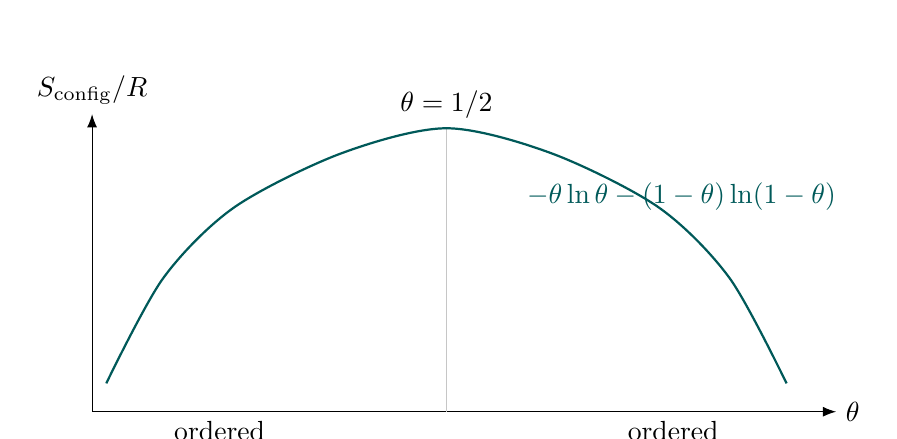
\begin{tikzpicture}[x=9.0cm,y=3.6cm,>=Latex]
  \draw[->] (0,0) -- (1.05,0) node[right] {$\theta$};
  \draw[->] (0,0) -- (0,1.05) node[above] {$S_\conf/R$};
  \draw[gray!45] (0.5,0) -- (0.5,1.0);
  \draw[thick,teal!70!black] plot[smooth] coordinates
    {(0.02,0.10) (0.10,0.47) (0.20,0.72) (0.35,0.91) (0.50,1.00)
     (0.65,0.91) (0.80,0.72) (0.90,0.47) (0.98,0.10)};
  \node[anchor=south] at (0.5,1.0) {$\theta=1/2$};
  \node[anchor=north] at (0.18,0) {ordered};
  \node[anchor=north] at (0.82,0) {ordered};
  \node[teal!70!black,anchor=west] at (0.60,0.76) {$-\theta\ln\theta-(1-\theta)\ln(1-\theta)$};
\end{tikzpicture}
\caption{Configurational entropy is the Shannon entropy of the occupied/empty site distribution.}
\label{fig:sconfig}
\end{figure}

\subsection{부분몰 항과 전위 온도 기울기}
Li 1몰을 더 넣을 때의 configurational 부분몰 entropy 는
\begin{equation}
\frac{\partial S_\conf}{\partial \theta}
=-R\ln\frac{\theta}{1-\theta}.
\label{eq:partial_config_theta}
\end{equation}
이제 Ch1 의 진행률 $\xi$ 를 \emph{탈리튬화 진행률}로 둔다. 즉 만충 쪽은
$\xi\to0$, 희박 Li 쪽은 $\xi\to1$ 이다. 이 convention 에서 logistic 전위 항은
\begin{equation}
V_j(\xi,T)=U_j(T)+\frac{RT}{F}\ln\frac{\xi}{1-\xi}
\label{eq:vxi}
\end{equation}
이고, 고정 $\xi$ 에서 온도로 미분하면
\begin{equation}
\frac{\partial V_j}{\partial T}\bigg|_{\xi}
=\frac{\partial U_j}{\partial T}
 \frac{R}{F}\ln\frac{\xi}{1-\xi}
=\frac{1}{F}\left[
\Delta S^0_{\rxn,j}+R\ln\frac{\xi}{1-\xi}\right].
\label{eq:config_in_dudt}
\end{equation}
여기서 $\Delta S^0_{\rxn,j}=F\,\partial U_j/\partial T$ 는
\emph{전이 중심} $\xi=1/2$ 의 표준 반응 entropy 다. 로그 항은 $\xi=1/2$ 에서
0 이고, 만충 한계 $\xi\to0$ 에서 $-\infty$, 희박 Li 한계 $\xi\to1$ 에서
$+\infty$ 로 간다.

\begin{keybox}
이중계산 금지: $\Delta S^0_{\rxn,j}$ 에 봉우리 내부 configurational entropy 를
다시 넣지 않는다. Ch1 의 $w=RT/F$ 와 식~\eqref{eq:vxi}가 이미
$R\ln[\xi/(1-\xi)]$ 를 생성한다. 따라서 $\Delta S^0_{\rxn,j}$ 는 중심 표준값,
configurational 항은 분포 폭에서 오는 별도 $x$-의존 항으로 분리한다.
\end{keybox}

% ====================================================================
\section{Vibrational 및 electronic entropy: 세 분포의 합}
\label{sec:vib_el}
% ====================================================================
\subsection{포논 Bose--Einstein 분포}
격자 진동은 포논 mode $k$ 의 Bose--Einstein 점유수
\begin{equation}
n_k^{\BE}=\frac{1}{\exp(\beta\hbar\omega_k)-1}
\label{eq:be}
\end{equation}
로 표현된다. harmonic mode 의 entropy 는
\begin{equation}
S_\vib
=R\sum_k\left[(1+n_k^{\BE})\ln(1+n_k^{\BE})
 -n_k^{\BE}\ln n_k^{\BE}\right].
\label{eq:svib}
\end{equation}
Li 삽입으로 graphite layer spacing, force constant, staging order 가 변하면
$\omega_k$ 분포가 바뀌고 $\Delta S_\vib$ 가 생긴다. 흑연에서는 저 Li 영역의
양의 configurational 항이 눈에 띄지만, 고 Li 영역에서는 진동 spectrum 변화가
음의 baseline 을 만들 수 있다 \cite{reynier2003,allart2018,jpcc2021}. Ch1 의
전이별 $\Delta S^0_{\rxn,j}$ 값은 이러한 느리게 변하는 vib 중심값을 포함한
표준 반응 entropy 로 취급한다.

\subsection{전자 Fermi--Dirac 분포}
전자 entropy 는 전자 상태밀도와 Fermi--Dirac 점유
\begin{equation}
f(E)=\frac{1}{\exp[(E-E_F)/\kB T]+1}
\label{eq:fd}
\end{equation}
에서 온다. 저온 금속 한계의 Sommerfeld 전개는
\begin{equation}
S_\el=\frac{\pi^2}{3}\kB^2T\,g(E_F)
\label{eq:sel}
\end{equation}
를 준다. 흑연 음극 하프셀에서는 이 항이 보통 configurational/vibrational 항보다
작다고 두는 것이 출발점이다. 그러나 Ch1 v9 에서 다룬 LCO 같은 단일 전극 하프셀의
metal-insulator-transition gate 에서는 $g(E_F)$ 가 조성에 따라 크게 변하고,
삽입 기준 $\Delta S_\el<0$ 인 electronic entropy 변화가 관측 $\partial U/\partial T$ 에
들어갈 수 있다. 이 장의 decomposition 은 그런 전극에도 같은 형식으로 적용된다.

\subsection{전이 내부 총 entropy 계수}
하나의 전이가 국소적으로 지배하는 영역에서 측정되는 entropy coefficient 는
\begin{equation}
\boxed{\;
\frac{\partial U}{\partial T}(\xi)
=\frac{1}{F}\Delta S(\xi),\qquad
\Delta S(\xi)=
\Delta S^0_{\rxn,j}
R\ln\frac{\xi}{1-\xi}
\Delta S_{\vib,j}^{\mathrm{slow}}(\xi)
\Delta S_{\el,j}^{\mathrm{slow}}(\xi)
\;}
\label{eq:decomp}
\end{equation}
로 정리한다. 실제 fitting 에서는 $\Delta S_{\vib}^{\mathrm{slow}}$ 와
$\Delta S_{\el}^{\mathrm{slow}}$ 가 전이 폭 안에서 천천히 변하면
$\Delta S^0_{\rxn,j}$ 에 흡수하고, 급격히 변하는 electronic gate 같은 경우에만
별도 $x$-의존 함수로 둔다. 봉우리 내부의 급격한 로그 변화는
$\Delta S^0_{\rxn,j}(x)$ 를 억지로 함수화하지 않아도 분포가 자동으로 만든다.

% ====================================================================
\section{\texorpdfstring{겹침과 mixing: 계단이 아니라 국소 $dQ/dV$ 가중 평균}{겹침과 mixing: 계단이 아니라 국소 dQ/dV 가중 평균}}
\label{sec:mixing}
% ====================================================================
\subsection{음함수 미분}
여러 전이가 겹친 평형 전위는
\begin{equation}
\sum_j Q_j\,\xi_{\eq,j}(U_\oc,T)=Q\,x
\label{eq:implicit_ocv}
\end{equation}
를 만족하는 음함수로 볼 수 있다. 고정 $x$ 에서 온도로 미분하면
\begin{equation}
\frac{\partial U_\oc}{\partial T}\bigg|_x
=-\frac{\sum_j Q_j\,\partial \xi_j/\partial T|_{U}}
        {\sum_j Q_j\,\partial \xi_j/\partial U|_{T}}.
\label{eq:implicit_derivative}
\end{equation}
국소 peak shape 를
\begin{equation}
g_j=\frac{\partial \xi_j}{\partial U}
=\frac{\xi_j(1-\xi_j)}{w_j}
\label{eq:gj}
\end{equation}
로 두면, 중심 표준 entropy 만 보는 선두차수는
\begin{equation}
\boxed{\;
\frac{\partial U_\oc}{\partial T}(x)
=\frac{1}{F}\,
\frac{\sum_j Q_j\,g_j(x)\,\Delta S^0_{\rxn,j}}
     {\sum_j Q_j\,g_j(x)}
\;}
\label{eq:overlap_simple}
\end{equation}
이다. 즉 관측 $\partial U_\oc/\partial T$ 는 전이별 entropy coefficient 의 계단
함수가 아니라, 그 SOC 에서 실제로 열린 $dQ/dV$ peak 의 국소 비중
$Q_jg_j/\sum_kQ_kg_k$ 로 평균한 연속 함수다.

봉우리 내부 configurational 항까지 포함하면
\begin{equation}
\boxed{\;
\frac{\partial U_\oc}{\partial T}(x)
=\frac{1}{F}\,
\frac{\sum_j Q_jg_j(x)\left[\Delta S^0_{\rxn,j}
Rz_j(x)\right]}
{\sum_j Q_jg_j(x)},\qquad
z_j=\ln\frac{\xi_j}{1-\xi_j}
=\frac{U_\oc-U_j}{w_j}
\;}
\label{eq:overlap_full}
\end{equation}
가 된다. 식~\eqref{eq:overlap_simple}은 전이 중심값들의 mixing 을 보여주는
식이고, 식~\eqref{eq:overlap_full}은 다온도 OCV 차분으로 보는 전체
$\partial U/\partial T$ 에 대응한다.

\begin{figure}[t]
\centering
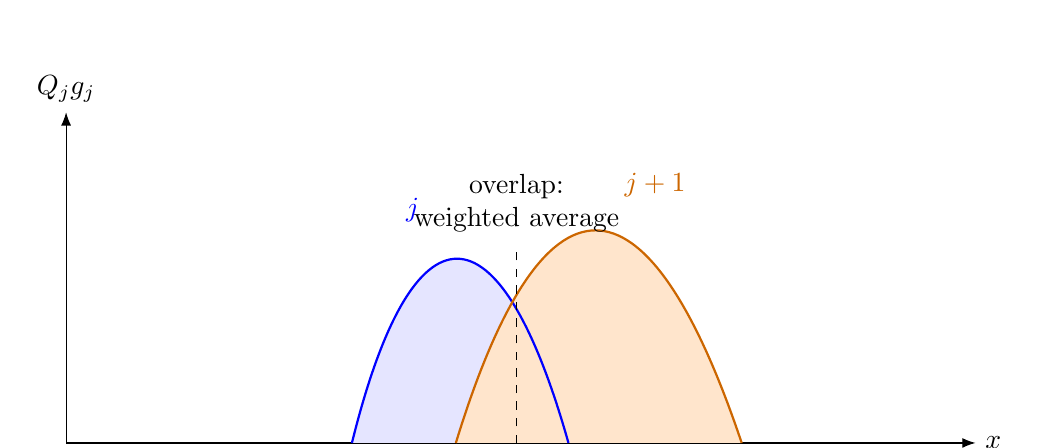
\begin{tikzpicture}[x=11.0cm,y=4.0cm,>=Latex]
  \draw[->] (0,0) -- (1.05,0) node[right] {$x$};
  \draw[->] (0,0) -- (0,1.05) node[above] {$Q_jg_j$};
  \fill[blue!10] (0.33,0) .. controls (0.40,0.78) and (0.50,0.78) .. (0.58,0) -- cycle;
  \fill[orange!20] (0.45,0) .. controls (0.55,0.90) and (0.67,0.90) .. (0.78,0) -- cycle;
  \draw[thick,blue] (0.33,0) .. controls (0.40,0.78) and (0.50,0.78) .. (0.58,0);
  \draw[thick,orange!80!black] (0.45,0) .. controls (0.55,0.90) and (0.67,0.90) .. (0.78,0);
  \draw[dashed] (0.52,0) -- (0.52,0.62);
  \node[blue] at (0.40,0.74) {$j$};
  \node[orange!80!black] at (0.68,0.82) {$j+1$};
  \node[align=center,anchor=south] at (0.52,0.64) {overlap:\\weighted average};
\end{tikzpicture}
\caption{When two staging peaks overlap, the entropy coefficient blends continuously with local $dQ/dV$ weights.}
\label{fig:overlap}
\end{figure}

\subsection{Numerical verification A}
The spine verification used the Ch1 four-transition graphite parameters and compared
finite-difference $U_\oc(x,T)$ between 292.15 K and 298.15 K with
equation~\eqref{eq:overlap_full}. The full expression matched the finite difference to
floating-point precision; the center-only expression had the expected residual because it
intentionally omits the $Rz_j/F$ configurational part. Representative values are:
\begin{center}
\small
\begin{tabular}{c c c c}
\toprule
$x$ & finite difference [mV/K] & center-only [mV/K] & full [mV/K]\\
\midrule
0.070 & $-0.3420$ & $-0.1455$ & $-0.3420$\\
0.450 & $-0.1113$ & $-0.1124$ & $-0.1113$\\
0.700 & $+0.0115$ & $-0.0667$ & $+0.0115$\\
0.930 & $+0.2790$ & $+0.1543$ & $+0.2790$\\
\bottomrule
\end{tabular}
\end{center}
The same check found no step discontinuity at transition boundaries: the observed
entropy coefficient moved continuously between neighboring $\Delta S^0_j/F$ values.

% ====================================================================
\section{Interaction width, hysteresis, and limits}
\label{sec:limits}
% ====================================================================
\subsection{\texorpdfstring{$w_\eff(\Omega)$}{weff(Omega)}}
For a Bragg--Williams regular solution, the equilibrium slope has the form
\begin{equation}
\frac{\dd V_\eq}{\dd \xi}
=\frac{RT}{F}\left[
\frac{1}{\xi(1-\xi)}-\frac{2\Omega}{RT}\right].
\label{eq:regular_slope}
\end{equation}
At $\xi=1/2$, the interaction term reduces the restoring curvature as
$\Omega$ approaches $2RT$. In the Ch1-style peak-width parameterization used for
capacity-domain transition kernels, the corresponding effective broadening is
\begin{equation}
\boxed{\;
w_\eff(\Omega)=\frac{w}{1-\Omega/(2RT)},\qquad \Omega<2RT.
\;}
\label{eq:weff}
\end{equation}
$\Omega=0$ recovers the ideal logistic width. As $\Omega\to2RT^-$, $w_\eff$ diverges:
the transition tends toward a plateau/two-phase limit, and the local entropy coefficient
is no longer a smooth single-site ideal mixing curve. If $\Omega$ has its own weak
temperature dependence, $\partial w_\eff/\partial T$ contributes a secondary correction
to $\partial U/\partial T$; this is a higher-order fitting term unless data demand it.

\begin{figure}[t]
\centering
\begin{tikzpicture}[x=9.0cm,y=4.0cm,>=Latex]
  \draw[->] (0,0) -- (1.05,0) node[right] {$\Omega/(2RT)$};
  \draw[->] (0,0) -- (0,1.08) node[above] {$w_\eff/w$};
  \draw[gray!45,dashed] (0.92,0) -- (0.92,1.02);
  \draw[thick,purple] plot[smooth] coordinates
    {(0.00,0.18) (0.20,0.23) (0.40,0.31) (0.60,0.45) (0.75,0.66)
     (0.84,0.85) (0.90,1.00)};
  \node[anchor=north] at (0.92,0) {$1$};
  \node[purple,anchor=west] at (0.47,0.62) {$1/[1-\Omega/(2RT)]$};
  \node[align=center,anchor=south east] at (0.88,0.93) {plateau\\limit};
\end{tikzpicture}
\caption{Interaction-renormalized transition width diverges as the regular-solution curvature approaches the spinodal limit.}
\label{fig:weff}
\end{figure}

\subsection{Hysteresis: reversible average and irreversible gap}
Hysteresis shifts the branch center. Write
\begin{equation}
U_j^{(d)}(T)=U_j^\rev(T)\pm\frac{1}{2}\Delta U_j^\hys(T),
\label{eq:hys_center}
\end{equation}
where $d$ denotes the charge or discharge branch. For each branch,
\begin{equation}
\frac{\partial U_\oc^{(d)}}{\partial T}
=\frac{1}{F}
\frac{\sum_j Q_jg_j^{(d)}
\left[\Delta S^{0,(d)}_{\rxn,j}+Rz_j^{(d)}\right]}
{\sum_j Q_jg_j^{(d)}}.
\label{eq:hys_branch}
\end{equation}
The reversible entropy coefficient used in $\dot Q_\rev$ is the branch average,
\begin{equation}
\frac{\partial U^\rev}{\partial T}
=\frac{1}{2}\left(
\frac{\partial U^\mathrm{ch}}{\partial T}
+\frac{\partial U^\mathrm{dis}}{\partial T}\right).
\label{eq:hys_rev}
\end{equation}
The voltage gap $\Delta U^\hys$ itself is not reversible entropy storage. It represents
history-dependent dissipative work and belongs with irreversible heat, roughly
$I\,\Delta U^\hys$ in the same sign convention as overpotential loss. Thus reversible
branch averaging and irreversible gap heating must be separated before interpreting
calorimetry or temperature-dependent OCV data \cite{hysteresis2018}.

\subsection{Corner limits}
\begin{longtable}{p{0.23\linewidth} p{0.47\linewidth} p{0.22\linewidth}}
\caption{Checks that keep the distribution model honest.}
\label{tab:limits}\\
\toprule
Limit & Entropy-coefficient behavior & Diagnostic\\
\midrule
\endfirsthead
\toprule
Limit & Entropy-coefficient behavior & Diagnostic\\
\midrule
\endhead
$\xi\to0$ (lithiated end) &
$R\ln[\xi/(1-\xi)]\to-\infty$; finite-size disorder and nonideal terms regularize measured data. &
Config divergence, no extra $\Delta S_j(x)$ needed.\\
$\xi\to1$ (Li-poor end) &
$R\ln[\xi/(1-\xi)]\to+\infty$; explains large positive low-Li graphite entropy. &
Matches $+29$ J mol$^{-1}$ K$^{-1}$ scale.\\
$\xi=1/2$ &
Config term is zero; $\partial U/\partial T=\Delta S^0_{\rxn,j}/F$ for an isolated transition. &
Defines center standard value.\\
$\Omega\to2RT^-$ &
$w_\eff\to\infty$ in the transition-width convention; plateau/two-phase behavior replaces ideal smooth mixing. &
Do not overfit with many fake peaks.\\
Single peak, no overlap &
Equation~\eqref{eq:overlap_full} reduces to equation~\eqref{eq:config_in_dudt}. &
Local consistency check.\\
High-temperature electronic gate &
$S_\el\propto T\,g(E_F)$ can become visible if $g(E_F)$ changes across the transition. &
Keep explicit only when electrode physics demands it.\\
\bottomrule
\end{longtable}

These limits state when the common approximation ``one constant $\Delta S^0_{\rxn,j}$ per
transition'' is valid. It is valid for the center standard part when vibrational and
electronic contributions vary slowly across the transition. It is not a claim that the
measured $\Delta S(x)$ is flat inside a peak. The measured nonlinearity comes from two
explicit sources already in the model: local overlap weighting and the configurational
log term.

% ====================================================================
\section{From entropy coefficient to reversible heat in coin half-cells}
\label{sec:qrev}
% ====================================================================
For a graphite coin half-cell at sufficiently low current, the operational workflow is:
\begin{workbox}
\begin{enumerate}[leftmargin=1.6em,itemsep=2pt]
\item Measure near-equilibrium charge/discharge or GITT/PITT-style OCV data at several
temperatures for the graphite electrode versus Li.
\item Fit the Ch1 transition model at each temperature or globally fit
$U_j(T)=U_j(T_0)+(T-T_0)\Delta S^0_{\rxn,j}/F$ with shared $Q_j$ and constrained widths.
\item Compute $g_j(x)$ and $\xi_j(x)$ from the fitted half-cell OCV, then evaluate
equation~\eqref{eq:overlap_full}.
\item Convert to reversible heat using
\[
\dot Q_\rev(x)=-I\,T\,\frac{\partial U_\oc}{\partial T}(x).
\]
\item Keep overpotential, ohmic loss, and hysteresis gap outside this reversible term.
\end{enumerate}
\end{workbox}

This is the v3 Bernardi chain, but with the missing distribution content filled in. The
same current can generate heating or cooling depending on the sign of
$\partial U_\oc/\partial T$. If the graphite electrode is in a low-Li, large positive
entropy region, the sign of $\dot Q_\rev$ follows equation~\eqref{eq:qrev_intro}; if it is
in a high-Li, negative entropy region, the reversible heat reverses sign. The sign is not
an empirical switch: it is the sign of the distribution reorganization entropy.

The $dQ/dV(T)$ route is useful because peak positions and overlaps carry the local
statistical weights. MSMR-style temperature parameterization provides a precedent for
estimating entropy coefficients from multi-reaction OCV models \cite{msmr_partI,msmr_partII},
while potentiometric entropy protocols provide the direct half-cell thermodynamic target
\cite{standardised2024}. The proposed graphite workflow differs by using the Chapter 1
$dQ/dV$ transition decomposition as the fitting coordinate.

% ====================================================================
\section{Measured graphite profile and literature anchoring}
\label{sec:profile}
% ====================================================================
The distribution equations must still meet measured graphite entropy. Published graphite
half-cell and electrode-resolved studies report a large positive entropy at low Li content
and negative values over much of the high-Li staging region \cite{reynier2003,allart2018}.
The Ch1 staging seed values,
\[
\Delta S^0_{\rxn,j}=\{+29,\;0,\;-5,\;-16\}\;
\mathrm{J\,mol^{-1}\,K^{-1}},
\]
therefore have the correct sign and scale for the graphite sequence. They should be read
as center standard values for transitions, not as the whole observed $\Delta S(x)$ curve.
The observed curve also contains equation~\eqref{eq:config_in_dudt} within each transition
and equation~\eqref{eq:overlap_full} where transitions overlap.

\begin{table}[t]
\centering\small
\renewcommand{\arraystretch}{1.15}
\caption{Graphite transition entropy values used as center standards in the half-cell model.}
\label{tab:ds}
\begin{tabular}{l c c c}
\toprule
Transition & Local region & Center $\Delta S^0_{\rxn,j}$ & Interpretation\\
\midrule
$4\to3$ & Li-poor side & $+29.0$ J mol$^{-1}$ K$^{-1}$ & large positive entropy scale\\
$3\to2\mathrm L$ & early staging & $0.0$ & center crossing/weak baseline\\
$2\mathrm L\to2$ & middle staging & $-5.0$ & negative vib-dominated trend\\
$2\to1$ & Li-rich side & $-16.0$ & high-Li negative entropy scale\\
\bottomrule
\end{tabular}
\end{table}

Enthalpy comparisons require care. Formation enthalpies for Li--graphite compounds and
differential transition enthalpies are not the same observable \cite{chemmater2015}.
This chapter uses $\Delta H_{\rxn,j}$ only through the Chapter 1 center voltage relation
$U_j(T)=(-\Delta H_{\rxn,j}+T\Delta S^0_{\rxn,j})/F$ and through the measured
temperature slope.

% ====================================================================
\section{Summary of the chapter logic}
\label{sec:summary}
% ====================================================================
\begin{enumerate}[leftmargin=1.6em,itemsep=3pt]
\item A Ch1 logistic transition is the two-state lattice-gas occupation distribution
from $Z_1=1+\exp[-\beta(\varepsilon_0-\mu)]$.
\item Configurational entropy is $S_\conf=-R\sum p\ln p$, giving the partial-molar log
term $R\ln[\xi/(1-\xi)]$ in $F\,\partial U/\partial T$.
\item $\Delta S^0_{\rxn,j}$ is the center standard value. It may include slowly varying
vibrational and electronic baseline terms, but it must not re-include the configurational
log term already generated by $w=RT/F$.
\item Overlap is a local $dQ/dV$ weighted average, not a step rule:
$Q_jg_j/\sum Q_kg_k$ is the weight.
\item $\Omega$ renormalizes transition width through
$w_\eff=w/[1-\Omega/(2RT)]$ until the plateau/two-phase limit invalidates the ideal
single-site smooth curve.
\item Hysteresis branch averaging belongs to reversible entropy; hysteresis gap heating
belongs to irreversible loss.
\item Reversible heat in the coin half-cell is
$\dot Q_\rev=-IT\,\partial U_\oc/\partial T=-(IT/F)\Delta S(x)$: heat associated with
distribution reorganization.
\end{enumerate}

% ====================================================================
\begin{thebibliography}{99}
\bibitem{bernardi1985} D. Bernardi, E. Pawlikowski, J. Newman, ``A General Energy Balance for Battery Systems,'' \emph{J. Electrochem. Soc.} \textbf{132}(1), 5--12 (1985). DOI: 10.1149/1.2113792.
\bibitem{newman} J. Newman, K. E. Thomas-Alyea, \emph{Electrochemical Systems}, 3rd ed., Wiley (2004). (OCV($T$): slope $=\Delta S$, intercept $=\Delta H$.)
\bibitem{reynier2003} Y. Reynier, R. Yazami, B. Fultz, ``The entropy and enthalpy of lithium intercalation into graphite,'' \emph{J. Power Sources} \textbf{119--121}, 850--855 (2003). DOI: 10.1016/S0378-7753(03)00285-4.
\bibitem{allart2018} D. Allart \emph{et al.}, ``Model of Lithium Intercalation into Graphite by Potentiometric Analysis with Equilibrium and Entropy Change Curves of the Graphite Electrode,'' \emph{J. Electrochem. Soc.} \textbf{165}(2), A380 (2018). DOI: 10.1149/2.1251802jes.
\bibitem{occupation2019} ``Transitions of lithium occupation in graphite: A physically informed model in the dilute lithium occupation limit supported by electrochemical and thermodynamic measurements,'' \emph{Electrochimica Acta} (2019). DOI: 10.1016/j.electacta.2019.135634. [method-level citation from v3 source list.]
\bibitem{chemmater2015} ``Intercalation Compounds from LiH and Graphite: Relative Stability of Metastable Stages\ldots,'' \emph{Chem. Mater.} \textbf{27} (2015). DOI: 10.1021/acs.chemmater.5b00235. [formation enthalpy context from v3 source list.]
\bibitem{jpcc2021} ``Thermodynamic Analysis of Li-Intercalated Graphite by First-Principles with Vibrational and Configurational Contributions,'' \emph{J. Phys. Chem. C} \textbf{125} (2021). DOI: 10.1021/acs.jpcc.1c08992. [abstract-tier support for vib/config decomposition.]
\bibitem{msmr_partI} ``Quantifying the Entropy and Enthalpy of Insertion Materials for Battery Applications Via the Multi-Species, Multi-Reaction Model,'' \emph{J. Electrochem. Soc.} (2024). DOI: 10.1149/1945-7111/ad1d27.
\bibitem{msmr_partII} ``Quantifying the Temperature Dependence of the MSMR Model Part II: Estimation of Entropy Coefficient for Meso-Carbon Micro-Bead Graphite,'' \emph{J. Electrochem. Soc.} (2024). DOI: 10.1149/1945-7111/ad70d9.
\bibitem{standardised2024} ``A Standardised Potentiometric Method for the Effective Parameterisation of Reversible Heating in a Lithium-Ion Cell,'' \emph{J. Electrochem. Soc.} (2024). DOI: 10.1149/1945-7111/ad4918.
\bibitem{hysteresis2018} ``Uncertainties in entropy due to temperature path dependent voltage hysteresis in Li-ion cells,'' \emph{J. Power Sources} (2018). DOI: 10.1016/j.jpowsour.2018.05.060.
\bibitem{huggins1942} M. L. Huggins, ``Theory of Solutions of High Polymers,'' \emph{J. Am. Chem. Soc.} \textbf{64}(7), 1712--1719 (1942). DOI: 10.1021/ja01260a068.
\bibitem{cogswell2012} D. A. Cogswell and M. Z. Bazant, ``Coherency Strain and the Kinetics of Phase Separation in LiFePO$_4$ Nanoparticles,'' \emph{ACS Nano} \textbf{6}(3), 2215--2225 (2012). DOI: 10.1021/nn204177u.
\bibitem{bazant2013} M. Z. Bazant, ``Theory of Chemical Kinetics and Charge Transfer based on Nonequilibrium Thermodynamics,'' \emph{Acc. Chem. Res.} \textbf{46}(5), 1144--1160 (2013). DOI: 10.1021/ar300145c.
\end{thebibliography}

\end{document}
